% Provenance (never printed): cycle 4 SVT/physique, "La planete Terre,
% l'environnement": the ocean, its relief, its waters and their movements;
% see sources/book1/PROVENANCE.md. Book 1, grade 8, chapter 4.
% Vocabulary guard: owns the parts of the seafloor (one definition),
% salinity, ocean current (homograph: electric current -- link "ocean
% current" only), gyre. Ridge and trench were met as places in g7.1 (plate
% boundaries); seafloor spreading and subduction stay there. The deep
% circulation is told (no "thermohaline" definition: Book 2).
\chapter{De oceanen}\label{ch:g8:the-oceans}

In december 1872 vertrok een Brits marineschip, HMS \emph{Challenger}, uit
Engeland voor een reis van drieënhalf jaar rond de wereld. Zijn opdracht
was nieuw: uitzoeken wat er op de bodem van de \omterm{def:g2:water-on-earth:ocean}{oceanen} ligt. Keer op keer
stopte het schip op open \omterm{def:g2:water-on-earth:ocean}{zee}, en de bemanning liet een zwaar gewicht aan
een lang touw zakken tot het de bodem raakte; de lengte van het
uitgevierde touw gaf de diepte. Toen het schip in mei 1876 thuiskwam,
hadden zijn peilingen laten zien dat de oceaanbodem diepe \omterm{def:g1:landscapes-around-us:landform}{vlakten} en grote
bergketens heeft.
% ledger: nhm:challenger-voyage, edin:challenger-stations

\begin{omfigure}
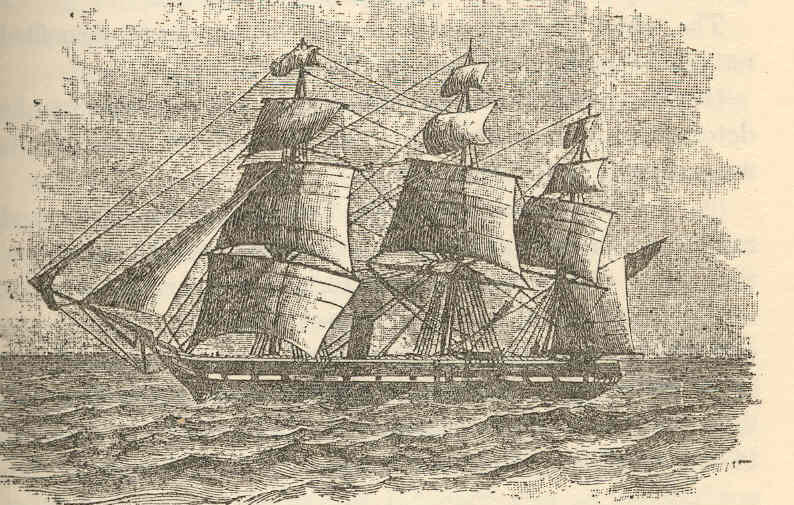
\includegraphics[width=0.55\linewidth]{images/book1/g8-challenger-sounding.jpg}

{\small HMS \emph{Challenger} maakt zich klaar om de diepte van de \omterm{def:g2:water-on-earth:ocean}{oceaan}
te peilen, 1872. Gravure uit de verslagen van de expeditie, overgenomen in
W.~A.~Herdman, \emph{Founders of Oceanography} (1923); publiek domein, via
Wikimedia Commons.}
% ledger: commons:challenger
\label{fig:g8:the-oceans:challenger}
\end{omfigure}

Tegenwoordig brengt een schip de zeebodem in \omterm{def:g2:drawing-to-map:map}{kaart} met geluid. Een
apparaat onder de romp zendt een korte geluidspuls naar beneden; het geluid
kaatst terug op de bodem en komt terug als een echo. De tijd die de echo
nodig heeft, geeft de diepte, keer op keer, terwijl het schip doorvaart.
Dit is \emph{sonar}.
% ledger: nos:sonar

\begin{recall}
\omterm{def:g2:water-on-earth:salt-fresh}{Zout water} bedekt het grootste deel van de Aarde, in één wereldoceaan die
in \omterm{def:g2:water-on-earth:ocean}{oceanen} en \omterm{def:g2:water-on-earth:ocean}{zeeën} is verdeeld (\cref{ch:g2:water-on-earth}). \omterm{def:g7:plate-tectonics:plate}{Platen}
bewegen uit elkaar bij de \omterm{def:g8:the-oceans:seafloor}{oceanische ruggen}, en een \omterm{def:g7:plate-tectonics:plate}{plaat} zakt onder een
andere bij de troggen (\cref{ch:g7:plate-tectonics}). Boven de \omterm{def:g2:water-on-earth:ocean}{oceanen}
waaien de winden in grote gordels: \omterm{def:g8:winds-global-circulation:global-winds}{passaatwinden}, \omterm{def:g8:winds-global-circulation:global-winds}{westenwinden} en \omterm{def:g8:winds-global-circulation:global-winds}{polaire
oostenwinden}, afgebogen door de draaiing van de Aarde
(\cref{ch:g8:winds-global-circulation}).
\end{recall}

\section{De oceaanbodem}

Als het water van de \omterm{def:g2:water-on-earth:ocean}{oceanen} kon worden weggepompt, zou er een heel
verborgen \omterm{def:g1:landscapes-around-us:landscape}{landschap} tevoorschijn komen. Langs de \omterm{def:g1:landscapes-around-us:water}{kusten} loopt het land
onder de \omterm{def:g2:water-on-earth:ocean}{zee} door als een flauw hellend, ondiep plat. Dan duikt de bodem
langs een steile helling omlaag naar uitgestrekte, vlakke \omterm{def:g1:landscapes-around-us:landform}{vlakten},
kilometers diep. Uit deze \omterm{def:g1:landscapes-around-us:landform}{vlakten} rijzen bergketens op, en hier en daar
gaan smalle troggen dieper omlaag dan wat ook op Aarde.
% ledger: edin:challenger-stations

\begin{omfigure}
\begin{tikzpicture}[font=\footnotesize, >={Stealth[length=2mm]}]
  \fill[omSea] (0,0) rectangle (15.6,-4.2);
  \fill[omLithAlluv] (0,0.6) -- (1.2,0.15) -- (1.6,0) -- (3.4,-0.35)
    .. controls (3.9,-0.55) and (4.1,-2.6) .. (4.7,-3.1)
    -- (6.6,-3.35) -- (7.6,-3.1) -- (8.3,-2.2) -- (8.6,-1.7) -- (8.75,-1.9) -- (8.9,-1.65) -- (9.2,-2.3) -- (10.0,-3.15)
    -- (11.6,-3.4) -- (12.6,-3.45) -- (13.05,-4.1) -- (13.35,-3.0) -- (14.2,-0.9) -- (14.8,0.7) -- (15.6,1.3)
    -- (15.6,-4.6) -- (0,-4.6) -- cycle;
  \draw[black!70] (0,0.6) -- (1.2,0.15) -- (1.6,0) -- (3.4,-0.35)
    .. controls (3.9,-0.55) and (4.1,-2.6) .. (4.7,-3.1)
    -- (6.6,-3.35) -- (7.6,-3.1) -- (8.3,-2.2) -- (8.6,-1.7) -- (8.75,-1.9) -- (8.9,-1.65) -- (9.2,-2.3) -- (10.0,-3.15)
    -- (11.6,-3.4) -- (12.6,-3.45) -- (13.05,-4.1) -- (13.35,-3.0) -- (14.2,-0.9) -- (14.8,0.7) -- (15.6,1.3);
  \draw[omRiver] (1.55,0) -- (14.45,0);
  \node[anchor=south] at (8,0.05) {zeeniveau};
  \node[align=center] at (2.6,-0.85) {continentaal\\plat};
  \draw[->] (2.6,-0.55) -- (2.6,-0.25);
  \node[align=center, anchor=east] at (3.7,-2.0) {continentale\\helling};
  \draw[->] (3.75,-2.0) -- (4.1,-1.9);
  \node[align=center] at (5.7,-2.6) {abyssale vlakte};
  \node[align=center] at (8.75,-0.9) {oceanische rug};
  \draw[->] (8.75,-1.15) -- (8.75,-1.55);
  \node[align=center] at (11.1,-2.6) {abyssale vlakte};
  \node[align=center, anchor=west] at (13.5,-3.9) {diepzee-\\trog};
  \draw[->] (13.45,-3.9) -- (13.15,-3.9);
  \node[anchor=south] at (0.8,0.6) {continent};
  \node[anchor=south east] at (14.7,1.0) {gebergte};
\end{tikzpicture}

{\small De delen van de oceaanbodem, van een \omterm{def:g1:landscapes-around-us:water}{kust} naar de open \omterm{def:g2:water-on-earth:ocean}{oceaan} en
een andere \omterm{def:g1:landscapes-around-us:water}{kust} (een schets: diepten en breedten zijn niet op schaal).}
\label{fig:g8:the-oceans:sketch}
\end{omfigure}

\begin{definition}[De delen van de oceaanbodem]\label{def:g8:the-oceans:seafloor}
\begin{itemize}
  \item Het \emph{continentaal plat}\index{continentaal plat} is de
        ondiepe, flauw hellende rand van een \omterm{def:g3:continents-and-oceans:continent}{continent} onder de \omterm{def:g2:water-on-earth:ocean}{zee}.
  \item De \emph{continentale helling}\index{continentale helling} is de
        steile helling die van het plat naar de diepe oceaanbodem leidt.
  \item Een \emph{abyssale vlakte}\index{abyssale vlakte} is een
        uitgestrekt, heel vlak en diep deel van de oceaanbodem.
  \item Een \emph{oceanische rug}\index{oceanische rug} is een lange keten
        van onderzeese \omterm{def:g1:landscapes-around-us:landform}{bergen} die uit de abyssale \omterm{def:g1:landscapes-around-us:landform}{vlakten} oprijst.
  \item Een \emph{diepzeetrog}\index{diepzeetrog} is een lange, smalle en
        heel diepe geul in de oceaanbodem, vaak naast een keten van \omterm{def:g1:landscapes-around-us:landform}{bergen}
        of vulkanische eilanden.
\end{itemize}
\end{definition}
% ledger: edin:challenger-stations, usgs:trench-depth

De \omterm{def:g2:water-on-earth:ocean}{oceaan} is gemiddeld ongeveer \qty{3700}{m} diep, bijna de helft van de
hoogte van de hoogste \omterm{def:g1:landscapes-around-us:landform}{berg} op het land. Zijn diepste punt, de
Challengerdiepte in de Marianentrog in de Stille \omterm{def:g2:water-on-earth:ocean}{Oceaan}, ligt bijna
\qty{11000}{m} onder het oppervlak.
% ledger: nos:ocean-depth, usgs:trench-depth, tht:everest


\begin{method}[Een profiel van de oceaanbodem lezen]
\begin{enumerate}
  \item Lees de assen: de afstand in de breedte, de hoogte of diepte op en
        neer, en de verticale overdrijving.
  \item Zoek het \omterm{def:g4:world-physical-map:altitude}{zeeniveau} (hoogte 0) en de \omterm{def:g1:landscapes-around-us:water}{kusten} waar het profiel het
        snijdt.
  \item Volg de bodem vanaf een \omterm{def:g1:landscapes-around-us:water}{kust}: het ondiepe plat, de steile helling,
        dan de diepe, vlakke \omterm{def:g1:landscapes-around-us:landform}{vlakten}.
  \item Zoek wat uit de \omterm{def:g1:landscapes-around-us:landform}{vlakten} oprijst (een rug) of eronder wegzakt (een
        trog), en lees de diepte ervan af.
\end{enumerate}
\end{method}

\begin{example}[Dwars door de zuidelijke Atlantische Oceaan]
Op het bovenste profiel daalt de bodem voorbij de \omterm{def:g1:landscapes-around-us:water}{kust} van Zuid-Amerika in
minder dan \qty{300}{km} tot meer dan \qty{3000}{m} diepte. \omterm{def:g8:the-oceans:seafloor}{Abyssale
vlakten}, tussen \qty{3500}{m} en \qty{5000}{m} diep, vullen het grootste
deel van de breedte. Halverwege, ongeveer \qty{4400}{km} langs het profiel,
rijst de Midden-Atlantische Rug op tot ongeveer \qty{2300}{m} onder het
oppervlak: meer dan \qty{2000}{m} boven de \omterm{def:g1:landscapes-around-us:landform}{vlakten}, een bergketen die
onder de \omterm{def:g2:water-on-earth:ocean}{zee} verborgen ligt. De \omterm{def:g1:landscapes-around-us:landform}{vlakten} worden weer dieper dan
\qty{5000}{m} voordat de bodem naar Afrika omhoogklimt.
\end{example}
% ledger: data:etopo1 (figdata/grade-8/seafloor_profile.py: ridge crest -2329 m at 4407 km; deepest -5295 m)

\begin{omfigure}
\begin{tikzpicture}
\begin{axis}[omsection, scale only axis, width=14cm, height=3.6cm, xmin=0, xmax=7569,
  ymin=-6000, ymax=1500, ytick={-6000,-4000,-2000,0}, xtick={0,1000,...,7000},
  xlabel={afstand langs 30.5\textdegree\ ZB, vanaf 59.5\textdegree\ WL (km)}, ylabel={hoogte (m)},
  tick label style={font=\scriptsize}, label style={font=\small},
  yticklabel style={/pgf/number format/1000 sep={\,}}, xticklabel style={/pgf/number format/1000 sep={\,}},
  axis background/.style={fill=white}, clip=true]
  \fill[omSea] (axis cs:0,-6000) rectangle (axis cs:7569,0);
  \addplot[fill=omLithAlluv, draw=black!70, line width=0.5pt] table[x=km, y=elev_m] {figdata/out/grade-8-seafloor_profile-atlantic-rock.dat};
  \node[font=\scriptsize, align=center, fill=white, inner sep=1pt] at (axis cs:4407,-900) {Midden-Atlantische Rug};
  \draw[-{Stealth[length=1.5mm]}] (axis cs:4407,-1250) -- (axis cs:4407,-2150);
  \node[font=\scriptsize] at (axis cs:2500,-5300) {abyssale vlakte};
  \node[font=\scriptsize] at (axis cs:6200,-5600) {abyssale vlakte};
  \node[font=\scriptsize, anchor=south west] at (axis cs:30,350) {Zuid-Amerika};
  \node[font=\scriptsize, anchor=south east] at (axis cs:7380,350) {Afrika};
  \node[anchor=north] at (rel axis cs:0.75,0.97) {\omve{260}};
\end{axis}
\end{tikzpicture}

\medskip
\begin{tikzpicture}
\begin{axis}[omsection, scale only axis, width=7cm, height=3.6cm, xmin=0, xmax=3020,
  ymin=-6000, ymax=4500, ytick={-6000,-4000,-2000,0,2000,4000}, xtick={0,1000,2000,3000},
  xlabel={afstand langs 20.5\textdegree\ ZB (km)}, ylabel={hoogte (m)},
  tick label style={font=\scriptsize}, label style={font=\small},
  yticklabel style={/pgf/number format/1000 sep={\,}}, xticklabel style={/pgf/number format/1000 sep={\,}},
  axis background/.style={fill=white}, clip=true]
  \fill[omSea] (axis cs:0,-6000) rectangle (axis cs:3020,0);
  \addplot[fill=omLithAlluv, draw=black!70, line width=0.5pt] table[x=km, y=elev_m] {figdata/out/grade-8-seafloor_profile-pacific-rock.dat};
  \node[font=\scriptsize, align=center, fill=white, inner sep=1pt] at (axis cs:1300,1600) {Peru-Chilitrog};
  \draw[-{Stealth[length=1.5mm]}] (axis cs:1750,1150) -- (axis cs:1870,-5000);
  \node[font=\scriptsize, anchor=west] at (axis cs:2600,3500) {Andes};
  \node[font=\scriptsize] at (axis cs:700,-5300) {abyssale vlakte};
  \node[anchor=north west] at (rel axis cs:0.01,0.98) {\omve{148}};
\end{axis}
\end{tikzpicture}

{\small Twee echte profielen van de oceaanbodem, afgelezen uit het reliëf
ETOPO1 bij elke \omterm{def:g6:latitude-longitude:longitude}{lengtegraad}. Boven: dwars door de zuidelijke Atlantische
\omterm{def:g2:water-on-earth:ocean}{Oceaan}, van Zuid-Amerika naar Afrika. Onder: dwars door de rand van
Zuid-Amerika aan de Stille \omterm{def:g2:water-on-earth:ocean}{Oceaan}. De hoogten zijn 260 en 148 keer
uitgerekt ten opzichte van de afstanden (\emph{verticale overdrijving}),
anders zou de \omterm{def:g2:water-on-earth:ocean}{oceaan} er zo dun uitzien als een vel papier; en met één punt
per graad lijkt de smalle trog minder diep dan hij is.}
% ledger: data:etopo1, earth:Rmean (figdata/grade-8/seafloor_profile.py)
\label{fig:g8:the-oceans:profiles}
\end{omfigure}


\section{Zout water}

Zeewater smaakt zout omdat er zouten in zijn opgelost. De meeste komen uit
de \omterm{def:g3:stones-pebbles-sand:rock}{gesteenten} van de \omterm{def:g3:continents-and-oceans:continent}{continenten}: \omterm{def:g4:clouds-rain-snow:precipitation}{regen} tast de \omterm{def:g3:stones-pebbles-sand:rock}{gesteenten} langzaam aan en
\omterm{def:g1:landscapes-around-us:water}{rivieren} voeren hun opgeloste zouten naar \omterm{def:g2:water-on-earth:ocean}{zee}. Sommige komen uit hete
bronnen op de oceaanbodem.
% ledger: nos:salinity-varies

\begin{definition}[Zoutgehalte]\label{def:g8:the-oceans:salinity}
Het \emph{zoutgehalte}\index{zoutgehalte} van zeewater is de massa zouten
die in een kilogram zeewater is opgelost. Gemiddeld is het ongeveer
\qty{35}{g} per kilogram: \qty{3.5}{\%} van de massa van zeewater is
zout.
\end{definition}
% ledger: nos:salinity-varies

Het \omterm{def:g8:the-oceans:salinity}{zoutgehalte} is niet overal gelijk. Als zeewater verdampt, verdwijnt
het water maar blijven de zouten achter: waar de zon fel is en \omterm{def:g4:clouds-rain-snow:precipitation}{regen}
zeldzaam, wordt de \omterm{def:g2:water-on-earth:ocean}{zee} zouter. Waar veel \omterm{def:g4:clouds-rain-snow:precipitation}{regen} valt, of waar een grote
\omterm{def:g1:landscapes-around-us:water}{rivier} uitmondt, is de \omterm{def:g2:water-on-earth:ocean}{zee} minder zout. Als zeewater bevriest tot zee-ijs,
blijft het zout achter in het water eromheen, dat daardoor ook zouter
wordt. Over het geheel is het \omterm{def:g8:the-oceans:salinity}{zoutgehalte} laag bij de \omterm{def:g3:continents-and-oceans:equator}{evenaar}, waar het
veel regent, en bij de \omterm{def:g3:continents-and-oceans:poles}{polen}; het is het hoogst op de middelste
breedten, onder de droge gordels rond \ang{30}.
% ledger: nos:salinity-varies, nos:sea-ice-salt, mo:three-cells

\begin{omfigure}
\begin{tikzpicture}[font=\footnotesize, >={Stealth[length=2mm]}]
  \fill[omSea] (0,0) rectangle (13,-1.6);
  \draw[omRiver, line width=0.8pt] (0,0) -- (13,0);
  % left: dry belt, evaporation
  \fill[yellow!80!orange] (1.2,3.0) circle (0.35);
  \foreach \x in {1.0,1.8,2.6,3.4} \draw[->, black!50, line width=0.9pt, decorate, decoration={snake, amplitude=0.6mm, segment length=3mm}] (\x,0.15) -- (\x,1.6);
  \node[align=center] at (2.3,2.2) {sterke verdamping,\\weinig regen};
  \node[align=center, fill=white, inner sep=1.5pt] at (2.3,-0.8) {\textbf{zouter}};
  % middle: rain
  \fill[black!20] (5.2,2.9) ellipse [x radius=1.3, y radius=0.4];
  \foreach \x in {4.4,4.8,...,6.0} \draw[omRiver] (\x,2.45) -- (\x-0.2,0.25);
  \node[align=center, fill=white, inner sep=1.5pt] at (5.2,-0.8) {\textbf{minder zout}};
  \node at (5.2,3.55) {zware regen};
  % right: river mouth and sea ice
  \fill[omLithAlluv] (7.4,0) -- (9.6,0) -- (9.6,0.6) -- (7.4,0.35) -- cycle;
  \draw[omRiver, line width=2pt, ->] (9.4,0.45) -- (7.9,0.2);
  \node[anchor=south] at (8.6,0.65) {rivier};
  \node[align=center, fill=white, inner sep=1.5pt] at (8.6,-0.8) {\textbf{minder zout}};
  \fill[white, draw=omCold] (10.6,0.25) -- (12.6,0.25) -- (12.4,-0.25) -- (10.8,-0.25) -- cycle;
  \node[anchor=south] at (11.6,0.3) {zee-ijs ontstaat};
  \node[align=center, fill=white, inner sep=1.5pt] at (11.6,-0.95) {\textbf{zouter}\\(zout blijft achter)};
\end{tikzpicture}

{\small Wat het \omterm{def:g8:the-oceans:salinity}{zoutgehalte} van de \omterm{def:g2:water-on-earth:ocean}{zee} verandert: verdamping en bevriezing
laten de zouten achter; \omterm{def:g4:clouds-rain-snow:precipitation}{regen} en \omterm{def:g1:landscapes-around-us:water}{rivieren} voegen \omterm{def:g2:water-on-earth:salt-fresh}{zoet water} toe.}
% ledger: nos:salinity-varies, nos:sea-ice-salt
\label{fig:g8:the-oceans:salinity}
\end{omfigure}

\begin{omfigure}
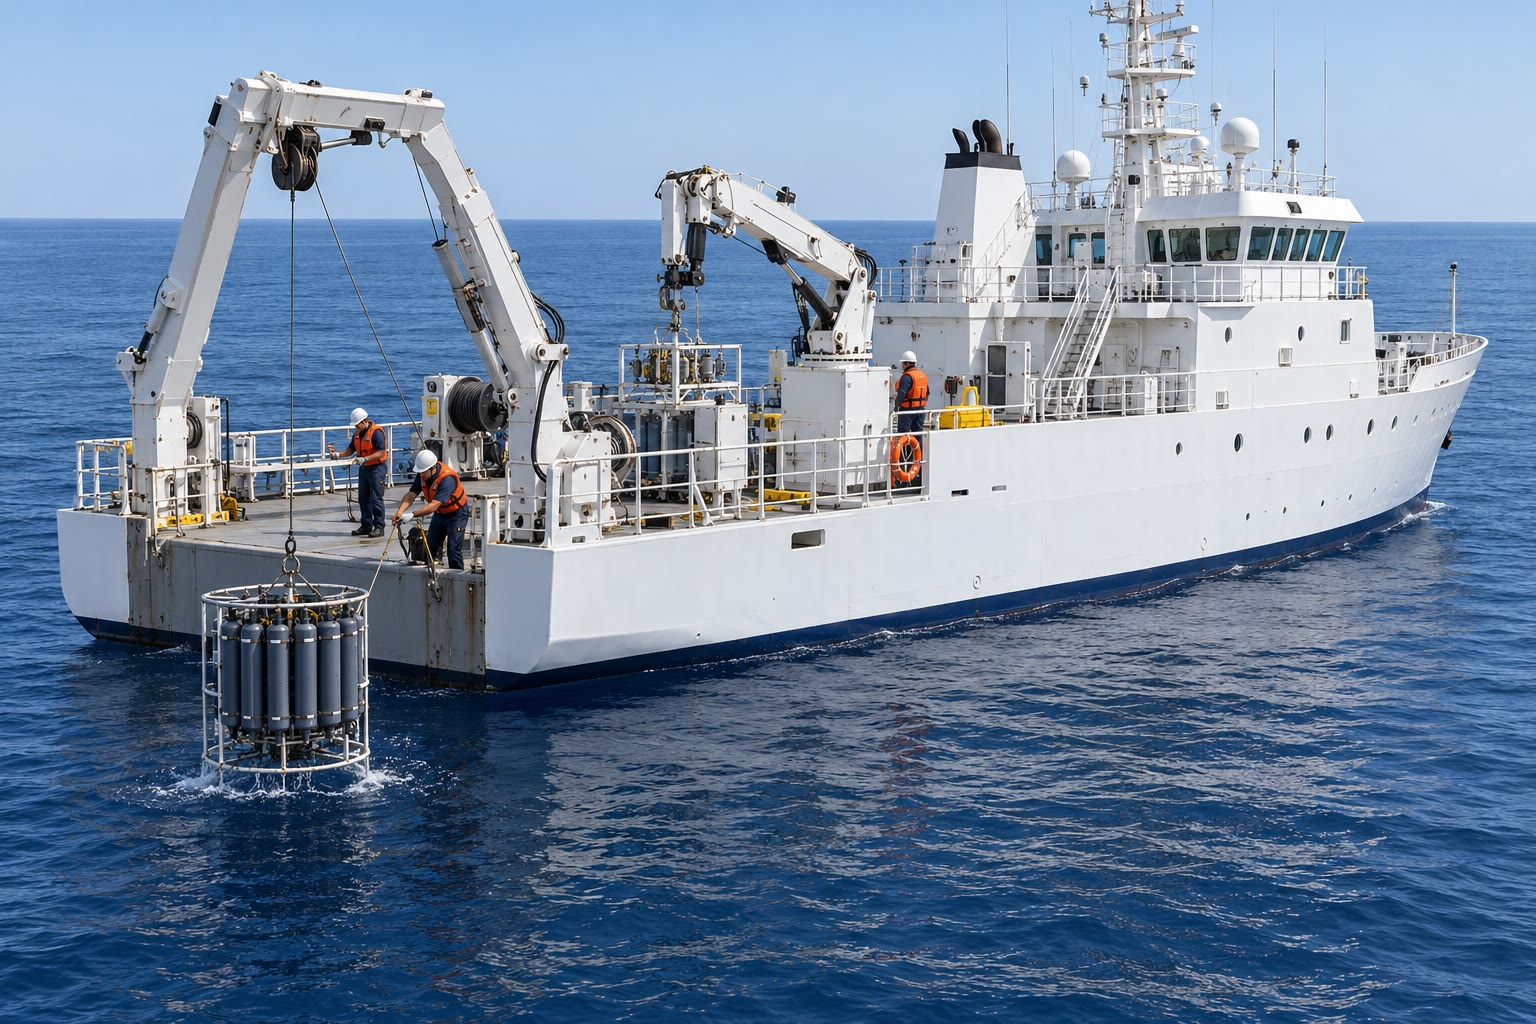
\includegraphics[width=0.58\linewidth]{images/book1/ai/g8-research-ship.jpg}

{\small Een onderzoeksschip laat een frame met monsterflessen in \omterm{def:g2:water-on-earth:ocean}{zee} zakken,
om water uit de diepte naar boven te halen en het \omterm{def:g8:the-oceans:salinity}{zoutgehalte} en de
temperatuur ervan te meten (door AI gegenereerde illustratie van een
algemene scène).}
\label{fig:g8:the-oceans:ship}
\end{omfigure}

\section{Stromingen aan het oppervlak}

De \omterm{def:g2:water-on-earth:ocean}{oceaan} is nooit stil. De winden trekken aan zijn oppervlak en zetten
het water in beweging: de gestage \omterm{def:g8:winds-global-circulation:global-winds}{passaatwinden} duwen het bij de \omterm{def:g3:continents-and-oceans:equator}{evenaar}
naar het westen, en de \omterm{def:g8:winds-global-circulation:global-winds}{westenwinden} duwen het op de middelste breedten naar
het oosten. Net als de winden wordt het bewegende water afgebogen door de
draaiing van de Aarde: naar rechts op het \omterm{def:g3:continents-and-oceans:equator}{noordelijk halfrond}, naar links
op het \omterm{def:g3:continents-and-oceans:equator}{zuidelijk halfrond}.
% ledger: nos:gyres

\begin{definition}[Zeestroming en gyre]\label{def:g8:the-oceans:current}
Een \emph{zeestroming}\index{zeestroming} is een gestage beweging van
zeewater in één richting, zoals een \omterm{def:g1:landscapes-around-us:water}{rivier} in de \omterm{def:g2:water-on-earth:ocean}{oceaan}. Een
\emph{gyre}\index{gyre} is een heel grote kringloop van zeestromingen die
rond een oceaanbekken draait.
\end{definition}
% ledger: nos:gyre-def, nos:gyres
\phantomsection\label{def:g8:the-oceans:gyre}

Er zijn vijf grote \omterm{def:g8:the-oceans:current}{gyres}: in de noordelijke en de zuidelijke Atlantische
\omterm{def:g2:water-on-earth:ocean}{Oceaan}, in de noordelijke en de zuidelijke Stille \omterm{def:g2:water-on-earth:ocean}{Oceaan}, en in de
Indische \omterm{def:g2:water-on-earth:ocean}{Oceaan}. Die van het \omterm{def:g3:continents-and-oceans:equator}{noordelijk halfrond} draaien met de klok mee,
die van het \omterm{def:g3:continents-and-oceans:equator}{zuidelijk halfrond} tegen de klok in. Aan de westkant van elke
\omterm{def:g2:water-on-earth:ocean}{oceaan} is de stroming van de \omterm{def:g8:the-oceans:current}{gyre} smal en snel; aan de oostkant is ze
breed en langzaam.
% ledger: nos:gyres

\begin{inthelab}[Een gyre in een schaal]
Vul binnen een grote ronde schaal met water en strooi een snufje peper op
het oppervlak. Blaas met een rietje zacht en gelijkmatig over de schaal,
altijd in dezelfde richting, dicht bij een van de randen. Kijk naar de
peper: het water bij het oppervlak gaat met je adem mee bewegen, en al snel
draait het hele oppervlak in een kringloop rond de schaal.
\end{inthelab}

\begin{omfigure}
\begin{tikzpicture}
\begin{axis}[ommap, width=\linewidth, xmin=-180, xmax=180, ymin=-65, ymax=70,
  xtick={-180,-120,...,180}, ytick={-60,-30,0,30,60},
  xticklabels={$180^\circ$,$120^\circ$WL,$60^\circ$WL,$0^\circ$,$60^\circ$OL,$120^\circ$OL,$180^\circ$},
  yticklabels={$60^\circ$ZB,$30^\circ$ZB,$0^\circ$,$30^\circ$NB,$60^\circ$NB},
  tick label style={font=\scriptsize}]
  \addplot[fill=omLithAlluv, draw=black!45, line width=0.2pt] table {figdata/out/shared-geo-land.dat};
  \addplot[omWarm, line width=1.3pt] table {figdata/out/grade-8-ocean_currents-gyres-warm.dat};
  \addplot[omCold, line width=1.3pt] table {figdata/out/grade-8-ocean_currents-gyres-cold.dat};
  \addplot[quiver={u=\thisrow{u}, v=\thisrow{v}}, -{Stealth[length=2.6mm, width=2.2mm]}, omWarm, line width=1.3pt]
    table[x=lon, y=lat] {figdata/out/grade-8-ocean_currents-heads-warm.dat};
  \addplot[quiver={u=\thisrow{u}, v=\thisrow{v}}, -{Stealth[length=2.6mm, width=2.2mm]}, omCold, line width=1.3pt]
    table[x=lon, y=lat] {figdata/out/grade-8-ocean_currents-heads-cold.dat};
  \node[font=\scriptsize\bfseries, fill=white, inner sep=1pt, anchor=east] at (axis cs:-72,40) {Golfstroom};
  \node[font=\scriptsize\bfseries, fill=white, inner sep=1pt, anchor=west] at (axis cs:-12,25) {Canarische Str.};
\end{axis}
\end{tikzpicture}

{\small De vijf grote \omterm{def:g8:the-oceans:current}{gyres}, vereenvoudigd: met de klok mee op het
\omterm{def:g3:continents-and-oceans:equator}{noordelijk halfrond}, tegen de klok in op het zuidelijk. Rood: warme
stromingen, die uit de tropen komen; blauw: koude stromingen, die van
hogere breedten komen. De \omterm{def:g8:the-oceans:current}{gyre} van de noordelijke Atlantische \omterm{def:g2:water-on-earth:ocean}{Oceaan} wordt
in het westen begrensd door de Golfstroom en in het oosten door de
Canarische Stroom.}
% ledger: nos:gyres, data:ne-land (figdata/grade-8/ocean_currents.py)
\label{fig:g8:the-oceans:gyres}
\end{omfigure}

De bekendste van deze stromingen is de Golfstroom. Hij verlaat de Golf
van Mexico, loopt langs de \omterm{def:g1:landscapes-around-us:water}{kust} van Florida naar het noorden, buigt
ter hoogte van North Carolina af naar het oosten en steekt de Atlantische
\omterm{def:g2:water-on-earth:ocean}{Oceaan} over naar het noordoosten. Zijn warme water beweegt gemiddeld met
ongeveer \qty{6.4}{km} per uur, aan het oppervlak tot ongeveer
\qty{9}{km} per uur, en hij voert meer water mee dan alle \omterm{def:g1:landscapes-around-us:water}{rivieren} van de
wereld samen. Hij houdt de oostkust van Florida 's winters warmer en
brengt zachte lucht naar West-Europa.
% ledger: nos:gulf-stream, nos:gyres

\begin{omfigure}
\begin{minipage}[c]{0.5\linewidth}\centering
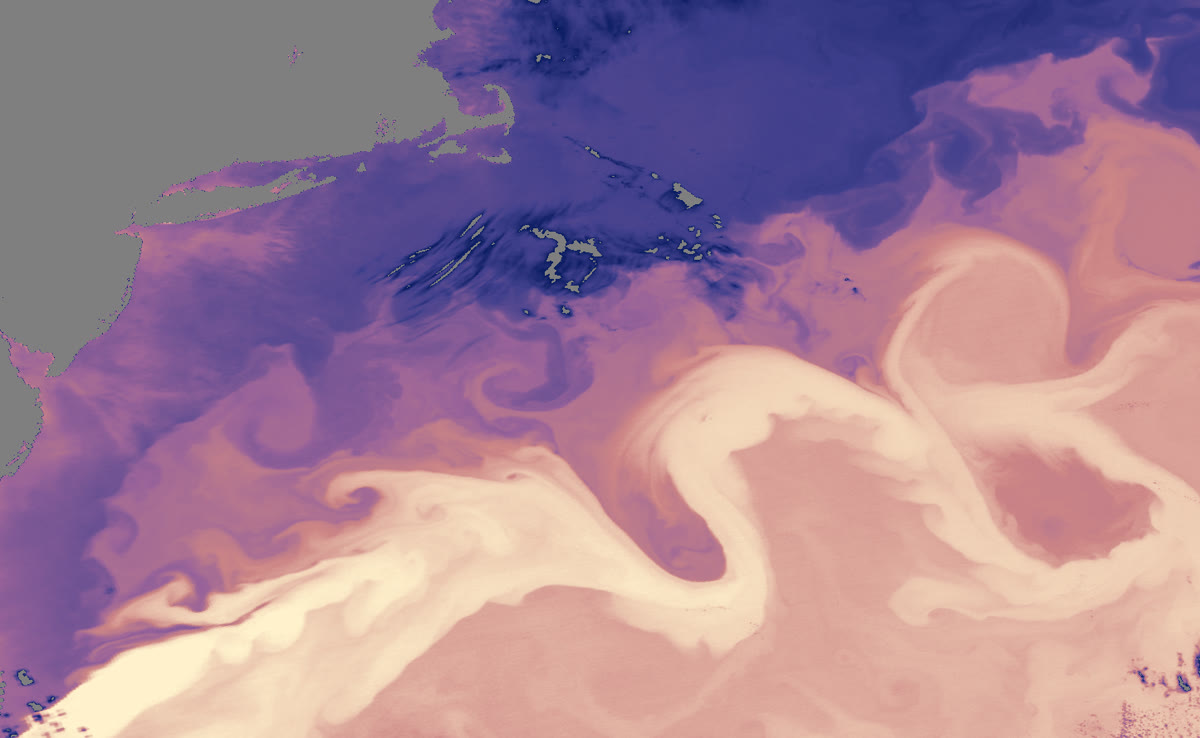
\includegraphics[width=\linewidth]{images/book1/g8-gulf-stream-sst.jpg}
\end{minipage}\hfill
\begin{minipage}[c]{0.46\linewidth}\raggedright
{\small De temperatuur van het zeeoppervlak voor de oostkust van
Noord-Amerika, gemeten door de satelliet Aqua van de NASA op 18~april
2005. De Golfstroom is de band van warm water (lichte kleuren, tot
ongeveer \qty{23}{\degreeCelsius}) die van linksonder naar rechts
kronkelt, tussen kouder water (donker, tot ongeveer
\qty{-1}{\degreeCelsius}); het land is grijs. NASA (publiek domein, via
Wikimedia Commons).}
\end{minipage}
% ledger: commons:gulf-sst
\label{fig:g8:the-oceans:gulf}
\end{omfigure}


\section{Diepe stromingen en de warmte van de oceaan}

De winden drijven de stromingen aan het oppervlak aan. Ver daaronder, in
de koude duisternis van de diepzee, beweegt het water ook, maar veel
langzamer. In het hoge noorden van de Atlantische \omterm{def:g2:water-on-earth:ocean}{Oceaan} geeft het warme
water dat de Golfstroom aanvoert zijn warmte af aan de koude lucht;
afgekoeld, en zouter geworden doordat er zee-ijs ontstaat, wordt het
dichter en zakt het naar de bodem. Dit koude, zoute water kruipt langs de
oceaanbodem naar het zuiden, helemaal tot Antarctica, en dan de Indische
en de Stille \omterm{def:g2:water-on-earth:ocean}{Oceaan} in, waar het langzaam opstijgt en aan het oppervlak
terugkeert. Een waterdruppel kan er ongeveer \num{1000} jaar over doen om
deze grote kringloop één keer rond te gaan: de \emph{grote oceanische
transportband}.
% ledger: nos:conveyor, nos:sea-ice-salt

\begin{omfigure}
\begin{tikzpicture}
\begin{axis}[ommap, width=\linewidth, xmin=-180, xmax=180, ymin=-65, ymax=70,
  xtick={-180,-120,...,180}, ytick={-60,-30,0,30,60},
  xticklabels={$180^\circ$,$120^\circ$WL,$60^\circ$WL,$0^\circ$,$60^\circ$OL,$120^\circ$OL,$180^\circ$},
  yticklabels={$60^\circ$ZB,$30^\circ$ZB,$0^\circ$,$30^\circ$NB,$60^\circ$NB},
  tick label style={font=\scriptsize}]
  \addplot[fill=omLithAlluv, draw=black!45, line width=0.2pt] table {figdata/out/shared-geo-land.dat};
  \addplot[omWarm, line width=1.3pt] table {figdata/out/grade-8-conveyor-surface.dat};
  \addplot[omCold, line width=1.3pt, dashed] table {figdata/out/grade-8-conveyor-deep.dat};
  \addplot[quiver={u=\thisrow{u}, v=\thisrow{v}}, -{Stealth[length=2.6mm, width=2.2mm]}, omWarm, line width=1.3pt]
    table[x=lon, y=lat] {figdata/out/grade-8-conveyor-heads-surface.dat};
  \addplot[quiver={u=\thisrow{u}, v=\thisrow{v}}, -{Stealth[length=2.6mm, width=2.2mm]}, omCold, line width=1.3pt]
    table[x=lon, y=lat] {figdata/out/grade-8-conveyor-heads-deep.dat};
  \node[font=\scriptsize\bfseries, fill=white, inner sep=1pt, anchor=west] at (axis cs:4,64) {zakt};
  \node[font=\scriptsize\bfseries, fill=white, inner sep=1pt, anchor=south] at (axis cs:163,11) {stijgt op};
\end{axis}
\end{tikzpicture}

{\small De grote oceanische transportband, vereenvoudigd tot één enkele
kringloop (een schets). Rood: warm water aan het oppervlak; blauw,
gestippeld: koud, \omterm{def:g2:water-on-earth:salt-fresh}{zout water} dat over de diepe oceaanbodem kruipt. Het
water zakt in het hoge noorden van de Atlantische \omterm{def:g2:water-on-earth:ocean}{Oceaan}, tussen Groenland
en Noorwegen, en stijgt op in de Stille \omterm{def:g2:water-on-earth:ocean}{Oceaan} (en, niet getekend, in de
Indische \omterm{def:g2:water-on-earth:ocean}{Oceaan}).}
% ledger: nos:conveyor, data:ne-land (figdata/grade-8/conveyor.py)
\end{omfigure}

\begin{example}[Hoe langzaam is het diepe water?]\label{ex:g8:the-oceans:deep-speed}
De kringloop op de \omterm{def:g2:drawing-to-map:map}{kaart} is ruwweg \qty{70000}{km} lang. Als een
waterdruppel er ongeveer \num{1000} jaar over doet om hem rond te gaan,
beweegt hij gemiddeld
ongeveer $\num{70000} \div \num{1000} = \qty{70}{km}$ per jaar, dat is
ongeveer \qty{200}{m} per dag. De Golfstroom legt met \qty{6.4}{km} per
uur ongeveer \qty{150}{km} per dag af: hij komt in ongeveer 11 uur even
ver als het diepe water in een heel jaar.
% ledger: nos:conveyor, nos:gulf-stream, earth:Rmean (loop length and speeds computed in figdata/grade-8/conveyor.py)
\end{example}

Samen voeren de stromingen aan het oppervlak en in de diepte warmte mee:
warm water stroomt van de tropen naar de \omterm{def:g3:continents-and-oceans:poles}{polen}, en koud water stroomt
terug naar de \omterm{def:g3:continents-and-oceans:equator}{evenaar}. Net als de winden vlakt de \omterm{def:g2:water-on-earth:ocean}{oceaan} de ongelijke
opwarming van de Aarde door de Zon af.
% ledger: nos:conveyor, nos:gulf-stream, mo:global-circ

\section{Oefeningen}

\begin{exercise}[$\star$]\label{exo:g8:the-oceans:1}
Zet deze delen van de oceaanbodem in de volgorde waarin een onderzeeër ze
tegenkomt als hij van een \omterm{def:g1:landscapes-around-us:water}{kust} naar het midden van de Atlantische \omterm{def:g2:water-on-earth:ocean}{Oceaan}
vaart: \omterm{def:g8:the-oceans:seafloor}{abyssale vlakte}; \omterm{def:g8:the-oceans:seafloor}{continentale helling}; \omterm{def:g8:the-oceans:seafloor}{oceanische rug};
\omterm{def:g8:the-oceans:seafloor}{continentaal plat}.
\end{exercise}

\begin{exercise}[$\star$]\label{exo:g8:the-oceans:2}
Waar of niet waar? Verbeter de onware zinnen. (a) De \omterm{def:g2:water-on-earth:ocean}{oceaan} is gemiddeld
ongeveer \qty{37}{km} diep. (b) De \omterm{def:g8:the-oceans:current}{gyres} van het \omterm{def:g3:continents-and-oceans:equator}{noordelijk halfrond}
draaien met de klok mee. (c) Verdamping maakt zeewater minder zout. (d) De
Golfstroom is een warme stroming.
\end{exercise}

\begin{exercise}[$\star$]\label{exo:g8:the-oceans:3}
Geef het woord bij elke beschrijving: (a) een lange keten van \omterm{def:g1:landscapes-around-us:landform}{bergen} onder
de \omterm{def:g2:water-on-earth:ocean}{zee}; (b) de massa zout in een kilogram zeewater; (c) een heel grote
kringloop van \omterm{def:g8:the-oceans:current}{zeestromingen}; (d) een lange, smalle en heel diepe geul in
de oceaanbodem.
\end{exercise}

\begin{exercise}[$\star$]\label{exo:g8:the-oceans:4}
Op de \omterm{def:g2:drawing-to-map:map}{kaart} van de \omterm{def:g8:the-oceans:current}{gyres}: (a) in welke richting draait de \omterm{def:g8:the-oceans:current}{gyre} van de
zuidelijke Atlantische \omterm{def:g2:water-on-earth:ocean}{Oceaan}? (b) Noem een warme en een koude stroming van
de noordelijke Atlantische \omterm{def:g2:water-on-earth:ocean}{Oceaan}. (c) Welke winden duwen het water bij de
\omterm{def:g3:continents-and-oceans:equator}{evenaar} naar het westen?
\end{exercise}

\begin{exercise}[$\star\star$]\label{exo:g8:the-oceans:5}
Een monster van \qty{1}{kg} zeewater bevat \qty{35}{g} zouten. (a)
Welk percentage van zijn massa is zout? (b) Hoeveel gram zouten zit er in
\qty{20}{kg} van dit water? (c) Hoeveel kilogram zeewater bevat
\qty{1}{kg} zouten?
\end{exercise}

\begin{exercise}[$\star\star$]\label{exo:g8:the-oceans:6}
De sonar van een schip zendt een geluidspuls recht naar beneden. De echo
komt \qty{6}{s} later terug. Geluid legt in zeewater ongeveer
\qty{1500}{m} per seconde af. (a) Hoe ver gaat het geluid in \qty{6}{s}?
(b) Waarom is de diepte maar de helft van deze afstand? (c) Wat is de
diepte? (d) Boven welk deel van de oceaanbodem zou het schip kunnen zijn?
\end{exercise}

\begin{exercise}[$\star\star$]\label{exo:g8:the-oceans:7}
Gebruik het profiel dwars door de zuidelijke Atlantische \omterm{def:g2:water-on-earth:ocean}{Oceaan}. (a) Hoe
diep liggen de \omterm{def:g8:the-oceans:seafloor}{abyssale vlakten} ongeveer? (b) Op welke afstand langs het
profiel ligt de top van de Midden-Atlantische Rug, en hoe diep ligt hij?
(c) Hoeveel meter rijst de rug boven de \omterm{def:g1:landscapes-around-us:landform}{vlakten} uit? (d) Waarom heeft het
profiel een verticale overdrijving nodig?
\end{exercise}

\begin{exercise}[$\star\star$]\label{exo:g8:the-oceans:8}
\omterm{def:g2:water-on-earth:ocean}{Zee} A ligt tussen twee \omterm{def:g5:weather-and-climate:desert}{woestijnen}: het regent er bijna nooit en er mondt
geen grote \omterm{def:g1:landscapes-around-us:water}{rivier} in uit. \omterm{def:g2:water-on-earth:ocean}{Zee} B, in een regenrijk gebied, ontvangt veel
grote \omterm{def:g1:landscapes-around-us:water}{rivieren}. Leg uit welke van de twee zouter is dan de open \omterm{def:g2:water-on-earth:ocean}{oceaan}, en
welke minder zout. Gebruik de woorden \emph{verdamping}, \emph{\omterm{def:g2:water-on-earth:salt-fresh}{zoet
water}}, \emph{zouten blijven achter}.
\end{exercise}

\begin{exercise}[$\star\star$]\label{exo:g8:the-oceans:9}
Voor de \omterm{def:g1:landscapes-around-us:water}{kust} van Florida wordt een flessenpost in \omterm{def:g2:water-on-earth:ocean}{zee} gegooid. (a) Welke
stroming voert hem eerst mee, en in welke richting? (b) In welke richting
steekt hij daarna de Atlantische \omterm{def:g2:water-on-earth:ocean}{Oceaan} over? (c) Langs welke \omterm{def:g1:landscapes-around-us:water}{kust} zou hij
naar het zuiden reizen als hij de \omterm{def:g8:the-oceans:current}{gyre} verder rondging? (d) Is deze
stroming warm of koud?
\end{exercise}

\begin{exercise}[$\star\star$]\label{exo:g8:the-oceans:10}
De Golfstroom beweegt gemiddeld met ongeveer \qty{6.4}{km} per uur. (a) Hoe
ver reist zijn water in één dag? (b) In een week? (c) Vergelijk met iemand
die \qty{5}{km} per uur wandelt.
\end{exercise}

\begin{exercise}[$\star\star\star$]\label{exo:g8:the-oceans:11}
De \omterm{def:g2:water-on-earth:ocean}{oceaan} is gemiddeld ongeveer \qty{3700}{m} diep, en zijn diepste punt
is bijna \qty{11000}{m} diep. (a) Schrijf beide diepten in kilometer.
(b) Hoeveel keer dieper dan het gemiddelde is het diepste punt? Rond af
op één decimaal. (c) Een sonarecho van het diepste punt: hoeveel seconden
doet hij erover om terug te komen, bij \qty{1500}{m} per seconde? (d) Een
waterdruppel van de transportband zakt in de noordelijke Atlantische
\omterm{def:g2:water-on-earth:ocean}{Oceaan}. Als hij er ongeveer \num{1000} jaar over doet om rond te gaan,
hoeveel jaar is dat als macht van tien?
\end{exercise}

\begin{exercise}[$\star\star\star$]\label{exo:g8:the-oceans:12}
De grote transportband van de diepzee begint in de Noorse \omterm{def:g2:water-on-earth:ocean}{Zee}, voor de
\omterm{def:g1:landscapes-around-us:water}{kust} van Noorwegen, waar warm water dat de Golfstroom aanvoert zijn warmte
afgeeft aan de koude lucht. (a) Leg met de \omterm{def:g2:drawing-to-map:map}{kaart} van de \omterm{def:g8:the-oceans:current}{gyres} en het
hoofdstuk stap voor stap uit hoe dit warme water vanuit de tropen daar is
gekomen, en welke winden het hebben voortgeduwd. (b) Leg uit waarom het
water daarna zakt. (c) Waar gaat het daarna naartoe?
\end{exercise}

\section{Probleem: Een drijvende boei}

\begin{problem}[{Weekendprobleem --- een drijvende boei wordt voor
Florida te water gelaten en rond de gyre van de noordelijke Atlantische
Oceaan meegevoerd; zijn reis wordt etappe voor etappe gevolgd, en de tijd
die hij nodig heeft om één keer rond te gaan wordt berekend}]
\label{pb:g8:the-oceans:1}
% ledger: nos:drifter, nos:gulf-stream, nos:gyres (figdata/grade-8/ocean_currents.py; the leg lengths are rounded, the speeds of legs B to D are exercise data)
Wetenschappers laten voor de \omterm{def:g1:landscapes-around-us:water}{kust} van Florida een drijvende boei te water.
Hij drijft net onder het oppervlak, beweegt met de stromingen mee en
stuurt zijn positie naar een satelliet. Zijn batterijen gaan ongeveer een
jaar mee. De \omterm{def:g2:drawing-to-map:map}{kaart} toont de vier etappes van zijn reis rond de \omterm{def:g8:the-oceans:current}{gyre} van de
noordelijke Atlantische \omterm{def:g2:water-on-earth:ocean}{Oceaan}.

\begin{center}
\begin{tikzpicture}
\begin{axis}[ommap, width=11.5cm, xmin=-95, xmax=0, ymin=5, ymax=55,
  xtick={-90,-60,-30,0}, ytick={10,30,50},
  xticklabels={$90^\circ$WL,$60^\circ$WL,$30^\circ$WL,$0^\circ$},
  yticklabels={$10^\circ$NB,$30^\circ$NB,$50^\circ$NB},
  tick label style={font=\scriptsize}]
  \addplot[fill=omLithAlluv, draw=black!45, line width=0.2pt] table {figdata/out/shared-geo-land.dat};
  \addplot[black, line width=1pt, densely dashed, postaction={decorate, decoration={markings,
      mark=between positions 0.04 and 0.98 step 0.08 with {\arrow{Stealth[length=2mm]}}}}]
    table[x=lon, y=lat] {figdata/out/grade-8-ocean_currents-buoy.dat};
  \addplot[only marks, mark=*, mark size=2.2pt, omDef] coordinates {(-79.5,26)};
  \node[font=\scriptsize\bfseries, anchor=east, fill=white, inner sep=1pt] at (axis cs:-81,26) {start};
  \addplot[only marks, mark=none, nodes near coords, point meta=explicit symbolic,
    every node near coord/.style={anchor=center, font=\footnotesize\bfseries, circle, fill=white, draw, inner sep=1pt}]
    table[x=lon, y=lat, meta=name] {figdata/out/grade-8-ocean_currents-buoy-legs.dat};
\end{axis}
\end{tikzpicture}

\medskip
{\small
\begin{tabular}{|c|l|c|c|}
\hline
etappe & stroming & lengte (km) & gemiddelde snelheid (km per dag) \\
\hline
A & Golfstroom & 3800 & 100 \\
B & Noord-Atlantische Stroom & 2100 & 20 \\
C & Canarische Stroom & 3100 & 20 \\
D & Noordequatoriale Stroom & 6100 & 20 \\
\hline
\end{tabular}}
\end{center}

\noindent\textbf{Deel I --- De lancering.}\par\nopagebreak
\begin{enumerate}[beginpenalty=10000]
  \item In welke \omterm{def:g2:water-on-earth:ocean}{oceaan}, en op welk \omterm{def:g3:continents-and-oceans:equator}{halfrond}, wordt de boei te water
        gelaten?
  \item In welke richting draait de \omterm{def:g8:the-oceans:current}{gyre}? Wordt de boei eerst naar het
        noorden of naar het zuiden meegevoerd?
  \item Is het water van etappe A warm of koud? En dat van etappe C? Leg
        uit.
  \item Welke winden drijven de stromingen van etappe B aan? En die van
        etappe D?
\end{enumerate}

\noindent\textbf{Deel II --- Rond de gyre.}\par\nopagebreak
\begin{enumerate}[resume, beginpenalty=10000]
  \item Hoeveel dagen duurt etappe A?
  \item Hoeveel dagen duren de etappes B, C en D?
  \item Wat is de totale lengte van de reis rond de \omterm{def:g8:the-oceans:current}{gyre}?
  \item Waarom is etappe A zoveel sneller dan de andere?
\end{enumerate}

\noindent\textbf{Deel III --- De duur van de reis.}\par\nopagebreak
\begin{enumerate}[resume, beginpenalty=10000]
  \item Hoeveel dagen heeft de boei nodig om één keer rond de \omterm{def:g8:the-oceans:current}{gyre} te gaan?
  \item Hoeveel maanden is dat, als je een maand op 30 dagen stelt? Rond af
        op een hele maand.
  \item Op welke etappe raken de batterijen leeg, na ongeveer een jaar
        (365 dagen)?
  \item Hoeveel maanden batterij zou de boei extra nodig hebben om zijn
        positie de hele weg rond te sturen?
\end{enumerate}
\end{problem}
